\chapter{Installation}
\label{ap: appendixA}

This appendix provides the steps for installing iBEMS on Ubuntu or any supported distribution of Linux.

\section{Cloning the repository}
The first step is to clone the repository with the command.
\begin{verbatim}
    git clone -b master https://github.com/ejwatkins
    /seniorProject1-2020-21-Code.git
\end{verbatim}
This will clone the master branch of the private Github repository owned by Elliot Watkins. It is recommended to run this command in the Unix user's home directory to find it easily.
\begin{figure}[H]
    \centering
    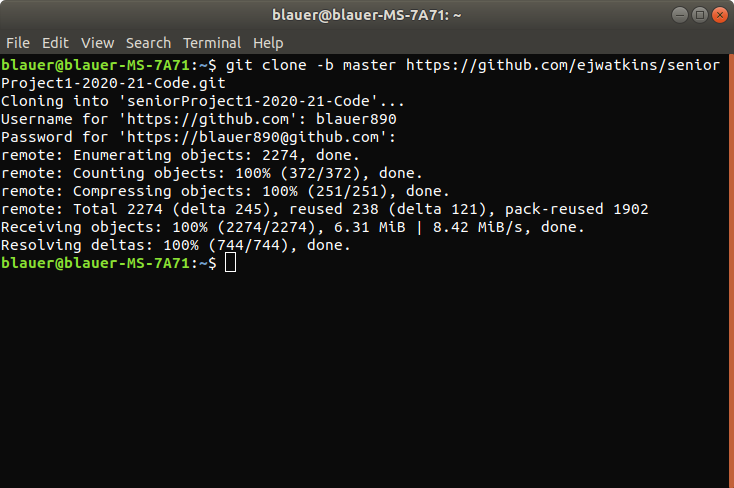
\includegraphics[scale=0.4]{figs/cloneiBEMS.png}
    \caption{Cloning iBEMS}
    \label{fig:cloneibems}
\end{figure}
If no errors occurred, terminal output similar to Figure~\ref{fig:cloneibems} will appear. A directory titled \texttt{seniorProject-2020-21-Code} will appear in the user's home directory.

\section{Creating the virtual environment}
Before the system can be properly installed, a Python 3 virtual environment must be created. After changing into the source code directory, this can be performed with the command
\begin{verbatim}
    python3 -m venv venv
\end{verbatim}
The final argument supplies the name of the directory the virtual environment will be placed in. For now, the name of the directory must be \texttt{venv} as this path name is hard coded in the source code. No terminal output should be generated when running this command if the proper version of Python 3 is installed along with the virtual environment package. If no errors occur, output similar to that of Figure~\ref{fig:createvenv} will be shown.

\begin{figure}[H]
    \centering
    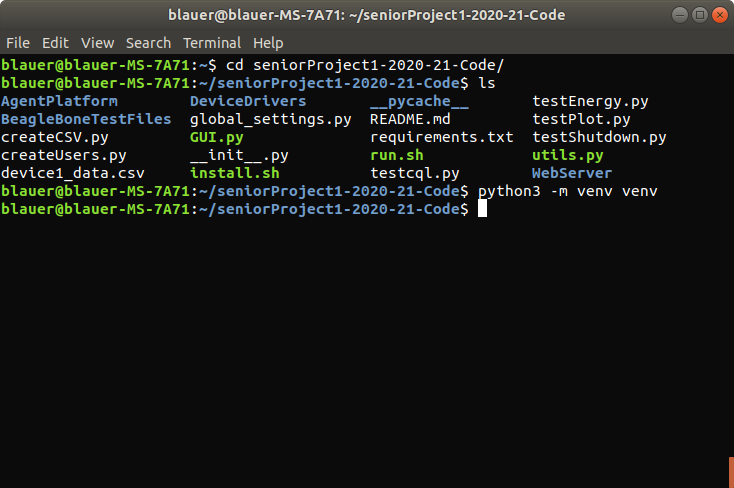
\includegraphics[scale=0.4]{figs/createvenv.png}
    \caption{Creating the virtual environment}
    \label{fig:createvenv}
\end{figure}

\section{Running the installation script}
Once the venv is created, the platform will be able to be properly installed by running the command
\begin{verbatim}
    ./install.sh
\end{verbatim}
If this script does not have executable permission for the current user, the following command will change the permissions of the file to allow it to be run by any normal user:
\begin{verbatim}
    chmod u+x install.sh
\end{verbatim}
This script will run through and install any necessary Python packages via the \texttt{requirements.txt} file, install the Apache Cassandra database, and place necessary project directories on the PYTHONPATH. Output similar to that in Figure~\ref{fig:runinstall} will be produced.

\begin{figure}[H]
    \centering
    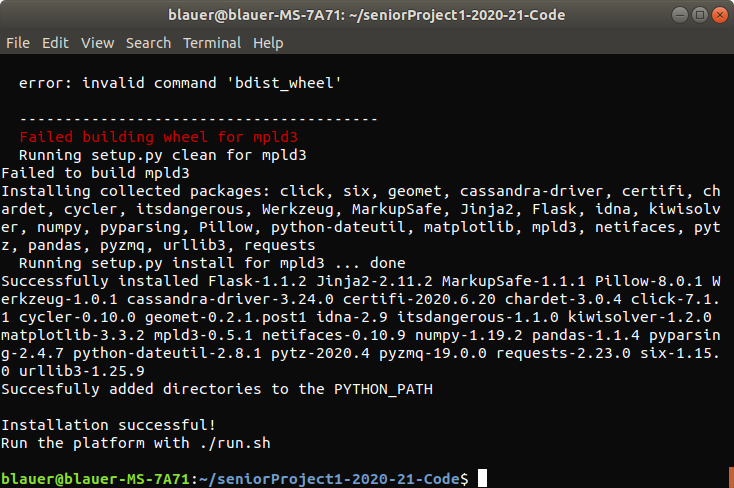
\includegraphics[scale=0.4]{figs/runinstall.png}
    \caption{Running the installation script}
    \label{fig:runinstall}
\end{figure}
An error regarding the installation of the \texttt{mpld3} package may be visible. However, this can be ignored as this package is not used in the current version of the software.
\medbreak\noindent
At this point, the software can be started with the \texttt{GUI.py} Python script.